\documentclass[tikz]{standalone}
\usepackage{tikz}
\usepackage[AutoFakeBold=true,AutoFakeSlant=true]{xeCJK}
\usepackage[zihao=-4,UTF8,heading=true]{ctex}
\usepackage[simplified]{pgf-umlcd}
\usetikzlibrary{fit} %形状
\usetikzlibrary{positioning} %不加方向运算可能出错
\usetikzlibrary{arrows.meta} %箭头
\usetikzlibrary{calc}

\setCJKmainfont{微软雅黑}
\begin{document}
	\thispagestyle{empty}
    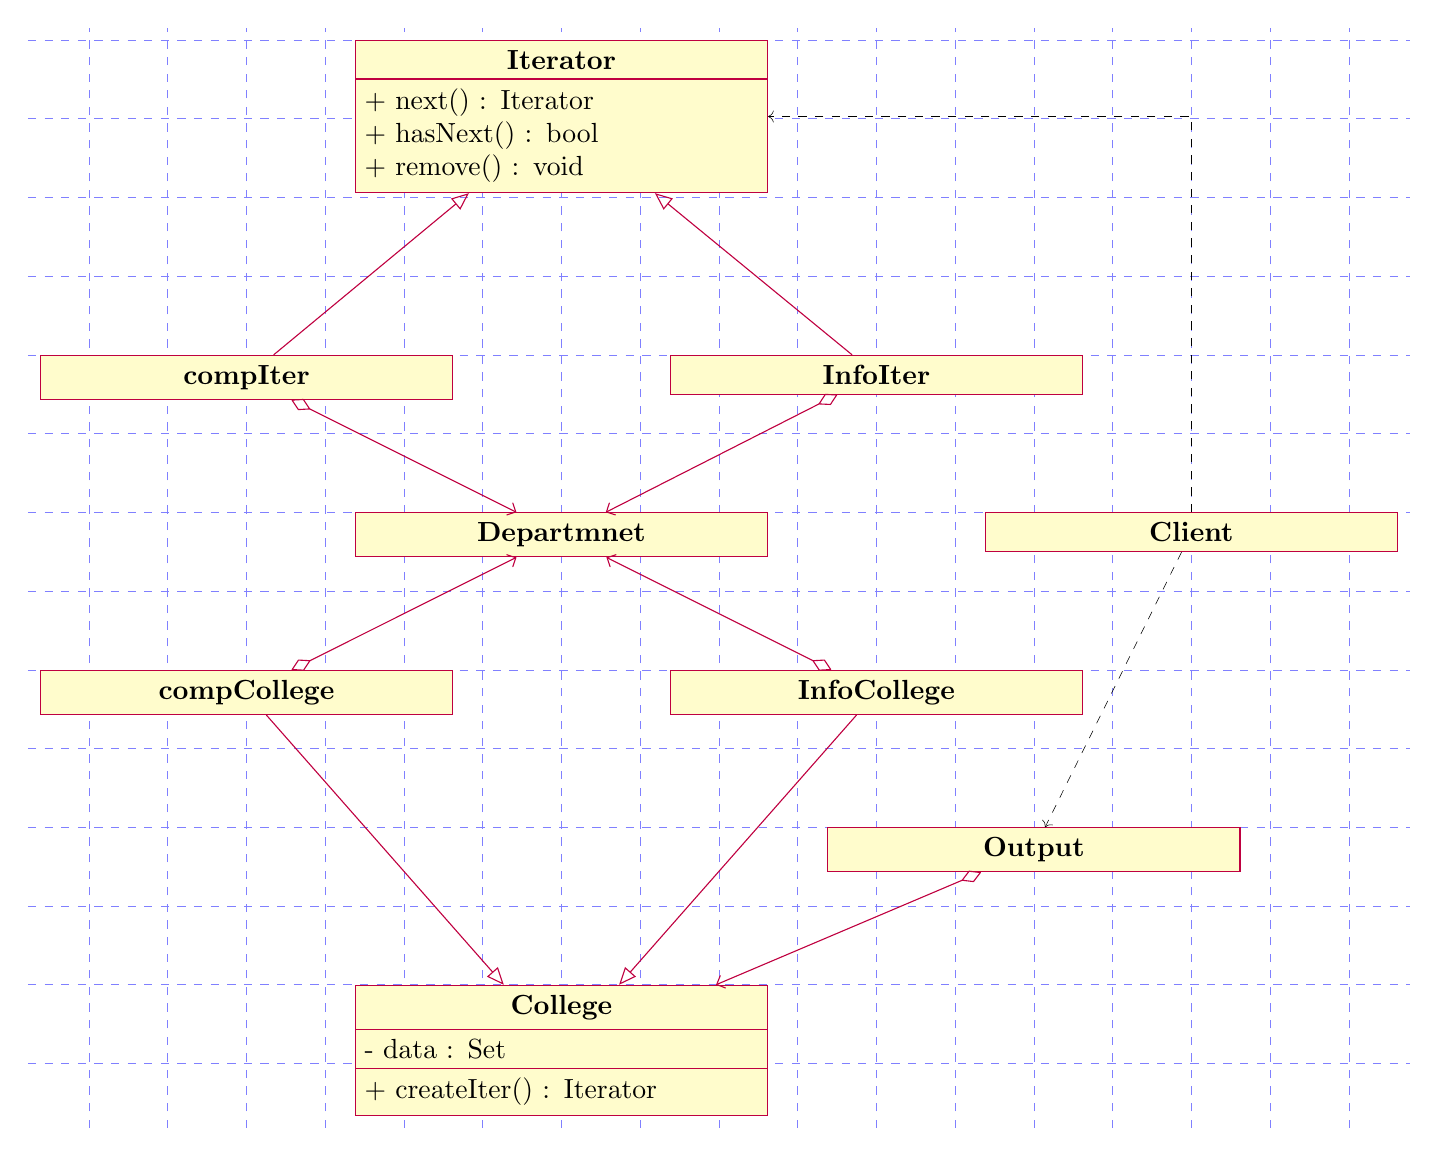
\begin{tikzpicture}[show background grid]
        \begin{class}[text width=5cm]{Iterator}{0,0}
            \operation{+ next() : Iterator}
            \operation{+ hasNext() : bool}
            \operation{+ remove() : void}
        \end{class}
        \begin{class}[]{compIter}{-4, -4}
            \inherit{Iterator}
        \end{class}
        \begin{class}[]{InfoIter}{4, -4}
            \inherit{Iterator}
        \end{class}
        
        \begin{class}[]{College}{0, -12}
            \attribute{- data : Set }
            \operation{+ createIter() : Iterator}
        \end{class}
        \begin{class}[]{compCollege}{-4,-8}
            \inherit{College}
        \end{class}
        \begin{class}[]{InfoCollege}{4, -8}
            \inherit{College}
        \end{class}
        \begin{class}[]{Departmnet}{0,-6} 
        \end{class}
        \aggregation{compIter}{}{}{Departmnet}
        \aggregation{InfoIter}{}{}{Departmnet}
        \aggregation{compCollege}{}{}{Departmnet}
        \aggregation{InfoCollege}{}{}{Departmnet}
        
        \begin{class}[]{Output}{6,-10}
        \end{class}
        \aggregation{Output}{}{}{College}
        \begin{class}[]{Client}{8,-6}
        \end{class}
        \draw [dashed,->,very thin] (Client) -- (Output);
        \draw [dashed,->,very thin] (Client) |- (Iterator);
        
    \end{tikzpicture}
    
    

\end{document}